 % !TEX encoding = UTF-8

\documentclass[12pt,a4paper,oneside]{article}

\usepackage[T1]{fontenc}
\usepackage[utf8x]{inputenc} %per usare e vedere le lettere accentate
\usepackage[english]{babel}
\usepackage[margin=2.5cm]{geometry}
\usepackage{setspace} %%per modificare interlinea
\onehalfspacing %%interlinea 1.5
\usepackage{pdfpages} %per aggiungere i file in pdf come il frontespizio
\pdfoptionpdfminorversion=7  %per eliminare warning sulla versione 1.7 del frontespizio
\usepackage{graphicx} %per aggiungere immagini
\graphicspath{{immagini/}} %path
\usepackage{flafter} % per impedire che le figure appaiano prima della loro citazione (attenzione: definirle cmq dopo la citazione)
\usepackage[font={small,it}]{caption} %per le didascalie delle figure (piccole e corsivo)
\usepackage[nottoc]{tocbibind} %per aggiugere la bibliografia all'indice (con numero di pagina)
\usepackage{url} %per usare url nella bibliografia
\usepackage{emptypage} %per evitare piè di pagina e testatine nelle pagine bianche
\usepackage{lmodern}
\usepackage[section]{placeins}  %per bloccare le figure nelle section e subsection relative (a fine section o subsection bisogna aggiungere \FloatBarrier)
\usepackage{cite}
\usepackage[listofformat=parens]{subfig} %per le sottofigure
% [listofformat=parens] serve per far comparire 1(a) quando uso \subref per chiamare la label della sottofig
\hyphenation{ImageNet label} %non voglio che vengano sillabate
\usepackage[english]{varioref} %cross-reference in italiano (figura tot a pagina tot)
\usepackage{adjustbox} %per poter aggiustare la tabella dell'architettura di vgg
\usepackage{amsmath}
\usepackage{algpseudocode}
\usepackage{algorithm}
\usepackage{algpseudocode}
\usepackage[pagebackref]{hyperref}

\makeatletter
\def\BState{\State\hskip-\ALG@thistlm}
\makeatother

\usepackage{fancyhdr}
\pagestyle{fancy}
\fancyhead{}
\renewcommand{\headrulewidth}{0pt}

\begin{document}
%\setcounter{secnumdepth}{5}
\setcounter{tocdepth}{5}
\setcounter{secnumdepth}{5}
\author{Nunzio Lopardo}
\date{\today}

\includepdf[pages={1}]{frontespizio.pdf}  
%\renewcommand{\figurename}{Figura} % cambio nome da Figure a Figura
%\renewcommand\contentsname{Indice} % rinomina indice
%\renewcommand{\cftsecleader}{\cftdotfill{\cftdotsep}} % per i punti nell'indice
% part\chapter\chapter\subchapter\subsubchapter\paragraph\subparagraph

%\frontmatter %pagine numerate con i numeri romani minuscoli e cap non numerati
\tableofcontents %%faccio comparire l'indice
\cleardoublepage %%interruzione di pagina

\section{Introduction}
\label{ch:intro}
This report describes the work to create an implementation of parallel $Breadth$-$First Search$ in order to find in a graph all the occurrences of an input value. In particular, has been implemented three solutions, two using the C++ STL and one using the Fast Flow library.


\section{Problem Analysis}
\label{ch:problem}
\subsection{Project Track}
\textit{A graph is described by a set of nodes N (with an associated value) and a set of arcs (oriented pairs of nodes). The application should take a node value X, a starting node S and must return the number of occurrences in the graph of the input node X found in the graph during a bread first parallel search starting from the node S. The graph to be searched is assumed to be acyclic.}

\subsection{Graph Generation}
\label{sec:graph}
For the creation of the graphs an algorithm has been developed taking into account the objectives of the project and also the available storage and computational capabilities. The algorithm is based on the Erdős-Rényi model and has been implemented in C++.

To manage the graph is used a $map<key, value>$, in which the key is the node $id$ and the values are instances of the class $Node$. This class is provided of all the properties of a node:

\begin{itemize}
    \item $int$ $id$;
    \item $atomic$<$bool$> $visited$;
    \item $atomic$<$bool$> $discovered$;
    \item $vector$<$Node*$> $neighbors$.
\end{itemize}

The generation procedure requires in input the desired number of nodes \textit{no\_nodes} and a \textit{density}, that indicates the probability to have an edge between each distinct couple of nodes.  The generation starts filling a $map\{int, Node*\}$ with all the nodes of the graph. The next step is the connection between the nodes taking into account the direct and acyclic nature of the graph. So for each node the algorithm iterate on other nodes with larger ids and generates a random value between 0 and 1, if the number is below the density values a link is established. 

For testing the solutions has been created 3 graphs:
\begin{itemize}
    \item 10000 nodes and 0.02 of density;
    \item 10000 nodes and 0.5 of density;
    \item 10000 nodes and 0.8 of density.
\end{itemize}

\subsection{Problem Analysis}
\label{sec:Problem_Analysis}
The \textit{Breadth-First Search} (BFS) is a graph visit algorithm, that takes in input a graph $G(V, E)$ and a starter node $v\in V$. The $BFS$ starts initializing the frontier vector $F$ with the starter's neighbors $v$ and an empty one called next frontier $F'$. In the next phase start the visit of the nodes in $F$, and for each node three operations are performed: 1) marking the node as visited, 2) check if has the same value as the input one, and 3) his list of neighbors is scanned to update the next frontier $F'$. Every time a new node is discovered is marked as $discovered$ and added to $F'$. When the visit of the frontier $F$ ends, it gets cleared and swapped with $F'$. The frontier visit and the swapping step are repeated until the next frontier $F'$ is empty. 

\begin{figure}[htb!]
    \centering
    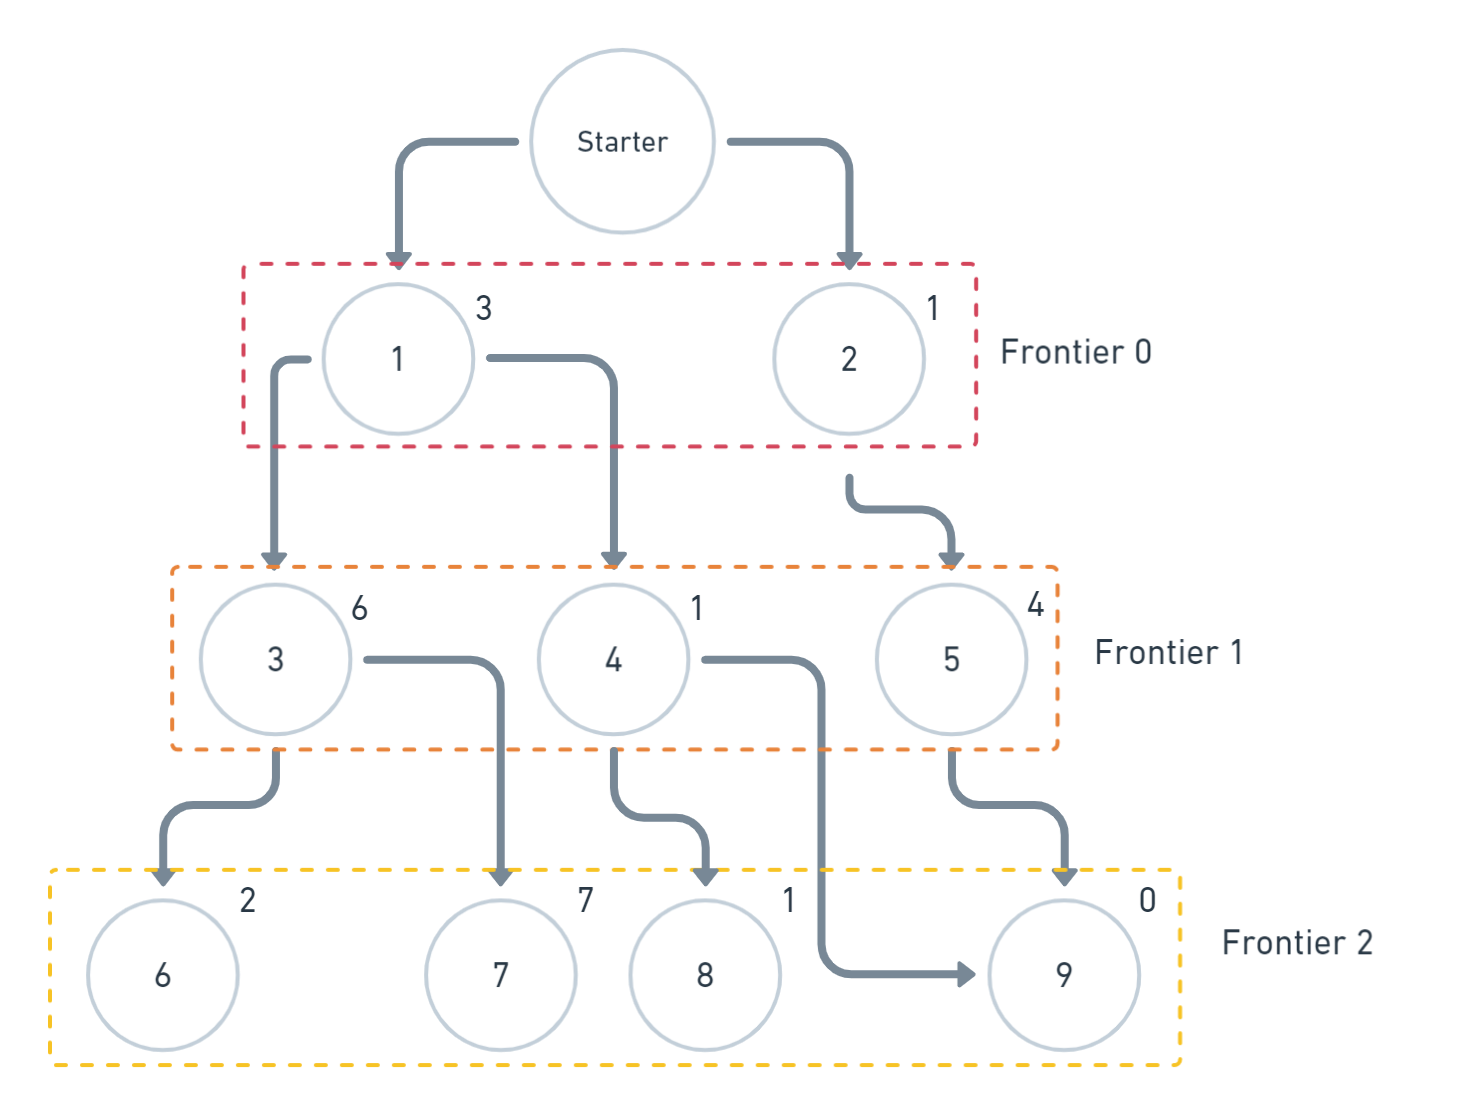
\includegraphics[width=0.58\textwidth]{Figures/seq_schema.png}
    \caption{Example of the BFS visit}
    \label{fig:bfs_tree}
\end{figure}
\FloatBarrier

\begin{figure}[htb!]
    \centering
    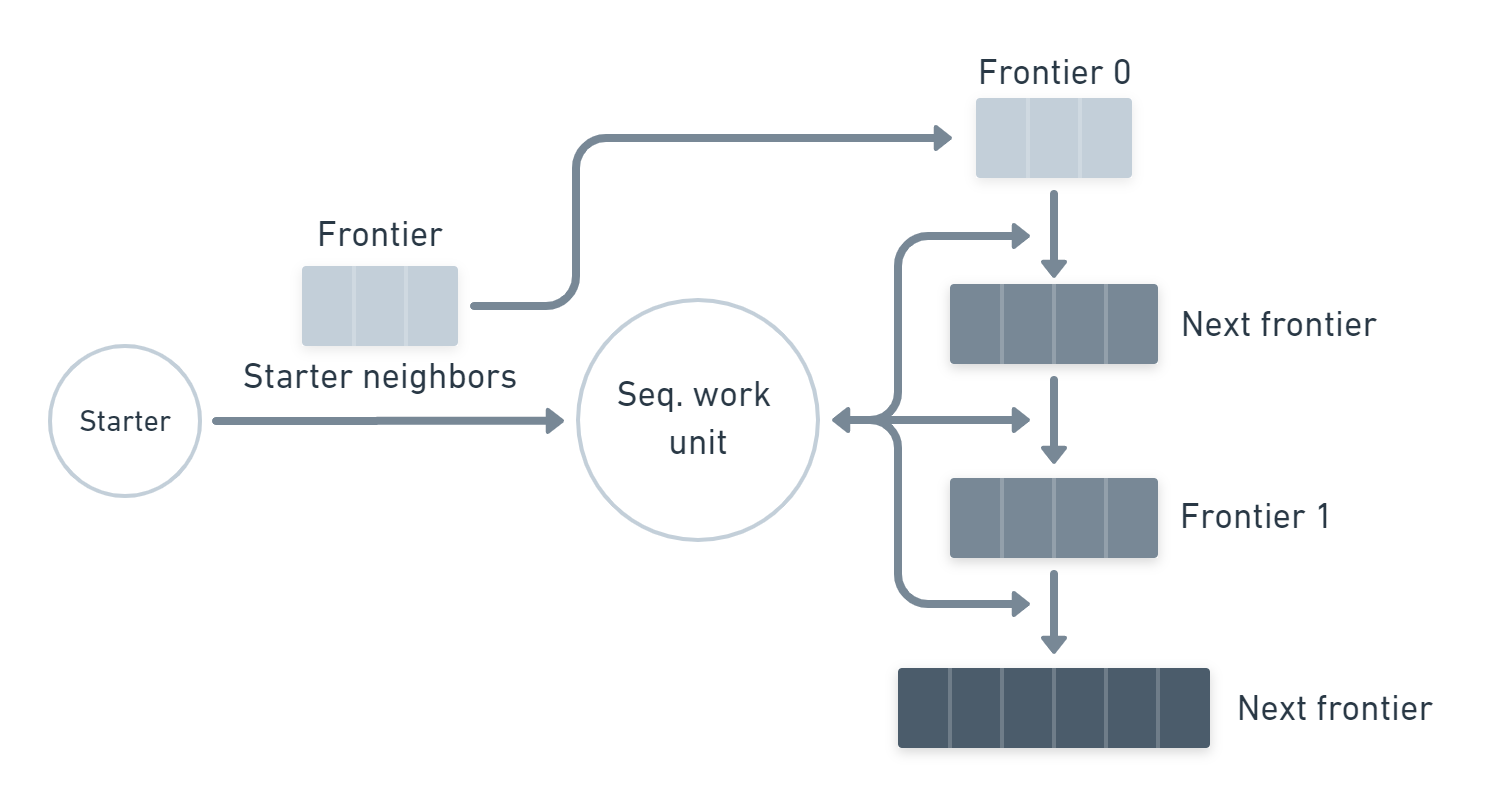
\includegraphics[width=0.8\textwidth]{Figures/seq_comp_schema.png}
    \caption{Schema of the sequential algorithm}
    \label{fig:bfs_seq_schema}
\end{figure}
\FloatBarrier

So in time terms the $BFS$ is performed as the sum (\ref{eq:T_seq}) of this two terms:

\begin{itemize}
    \item $T_{visit} (i)$ : as the time to visit a new i th frontier;
    \item $T_{swap}$: as the time to exchange the old with the new frontier.
\end{itemize}

\begin{equation}
\centering
T_{seq} = \displaystyle \sum_{i=0}^n T_{visit_i} + T_{swap}
\label{eq:T_seq}
\end{equation}

With $n$ as the number of frontiers and  $T_{visit_i} >>  T_{swap}$. Due to this last consideration the phase that lends itself best to be parallelized is frontier analysis. 
Considering to chose a farm-based approach and use $nw$ workers for visiting the frontier, we will obtain a visit time equal to $T_{visit}/nw$. However, to this, it is necessary to add the farm initialization time $T_{init}$, the time to divide and assign frontier chunks $T_e$ and the collecting time $T_c$. These last two terms replace the $T_{swap}$ of the sequential version.   
Thus the completion time of the parallel version will be:
\begin{equation}
\centering
T_{par} = T_{init} + \displaystyle \sum_{i=0}^n max\{T_e, T_{visit}/nw, T_c\}
\label{eq:T_par}
\end{equation}

It is necessary to say that everything depends on the properties of the graph, it makes sense to go for parallelization if you work with large frontiers in order to have $T_{visit}/nw >> T_{init} + T_e + T_c$. In fact, for graphs in which the degree of each node is very small, the disadvantages of parallelization will be greater than the benefits, this is due to the management of workers and synchronization in the merge phase of new frontiers. 



\section{Proposed Solutions}
\label{ch:solutions}
As mentioned in the \ref{sec:Problem_Analysis} the best spot of the execution to parallelize is the frontier scanning, this due to its huge size in most of graphs. To achieve this has been used a \textbf{farm pattern} in which the frontier is splitted among all the workers by an \textbf{emitter} and the results of worker computation are merged in a new frontier by a \textbf{collector}.
In all the following solutions the $nw$ is intended only as the number of workers in the farm, so are not considered the emitter and collector threads.
\subsection{C++ STL Solutions}
\label{subsec:CStatic}
\subsubsection{Static Scheduling}
In this section will be described in details the solution with the static scheduling of the frontier's chunks.
The execution starts with the initialization of the farm: an emitter, a vector of workers and a collector are created. In addition to this, are initialized all data structures for level analysis and synchronization. In particular, for communication, each worker has a queue where the emitter distributes chunk ranges. On the other hand, the data are retrieved from the farm exploiting shared references of the workers' new frontier with the collector.

With this approach, the emitter divides the frontier $F$ size by the number of workers ($nw$), then creates the pairs in which are present start and the end position of the chunk. These pairs are pushed in the worker's queue that extracts it and starts to work on his chunk. To avoid that the emitter execution restart a condition variable has been used to put the emitter thread in a wait state. 
Popped the chunk from the queue, the worker starts to iterate on the frontier in its range. For each node, firstly checks if the vertex has already been visited exploiting the $compare\_and\_exchange$ that allows to perform both fetch and update operations in an atomic fashion. The method returns true if it was able to change the state of the node to visit, otherwise, it is skipped.
In the case of a positive outcome, the analysis of the node continues by checking the value associated with it and visiting its list of neighbors. During this list iterations, is verified if the neighbor has been already added in the next frontier vector by another worker.
To synchronize the farm with the collector the workers perform a $fetch\_add$ operation on an atomic variable $end\_of\_task$, when it reaches $nw$ the collector operations start. In this phase all the workers' next frontiers are merged in $F'$, the old frontier $F$ gets cleared and swapped with $F'$. In addition, the condition variable state is changed to allow emitter restart. These three steps are repeated until the collector's next frontier is empty, in this case in the frontier is pushed a special node $Stopper$ received by the emitter that blocks the worker using $Stop\_exe$ pairs. When the worker receives this pair atomically fetch and add the local counter of the found occurrences to a shared counter.

\begin{figure}[htb!]
    \centering
    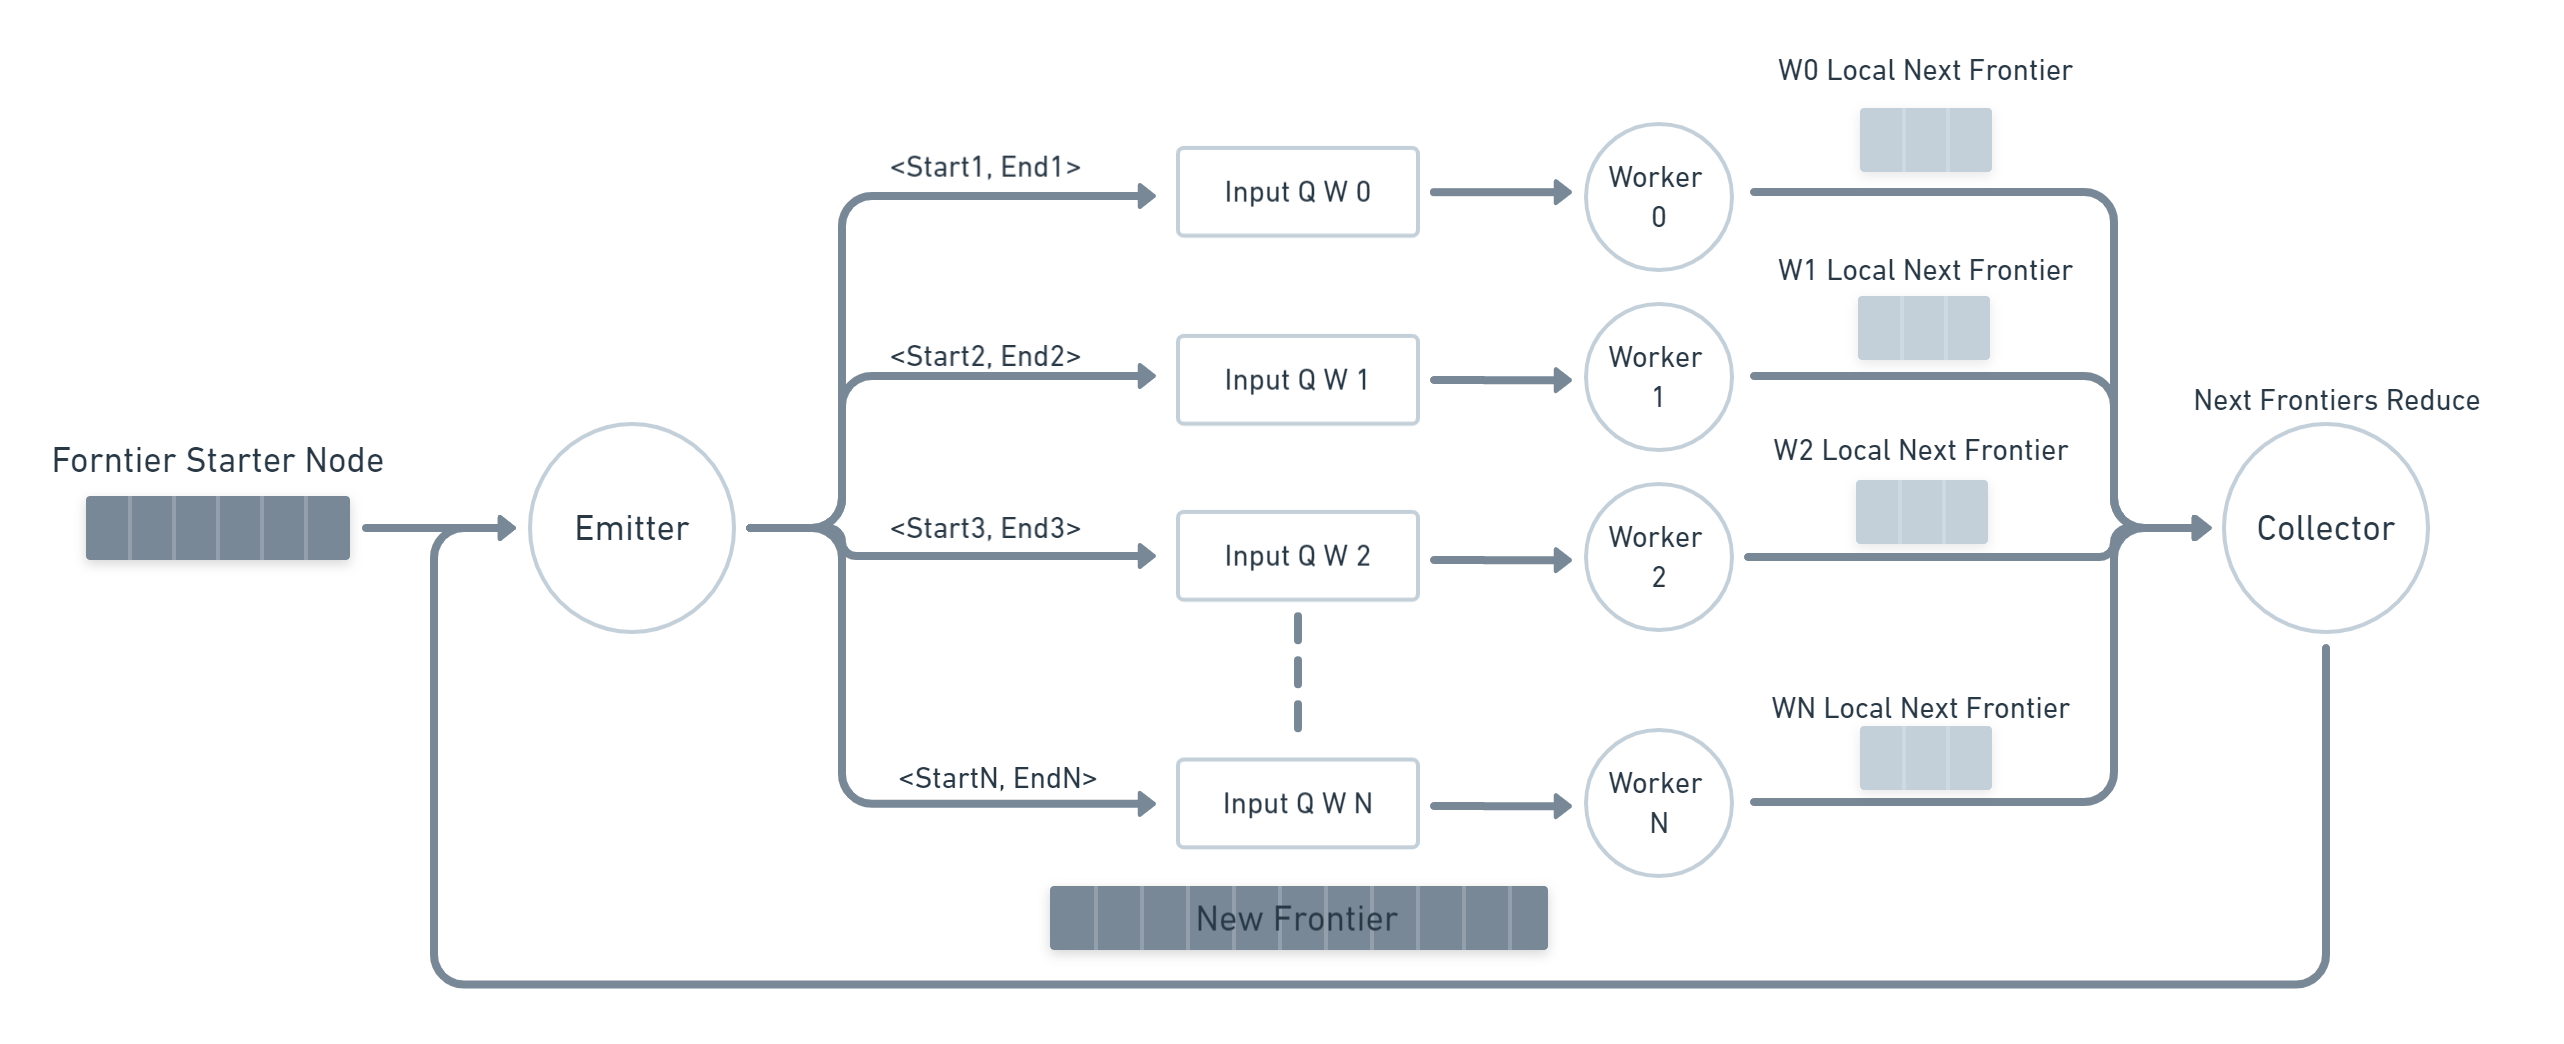
\includegraphics[width=0.95\textwidth]{Figures/par_schema.png}
    \caption{Schema of the static scheduling solution.}
    \label{fig:bfs_par_1_schema}
\end{figure}
\FloatBarrier

The main problem of this approach is the load balancing mostly in the cases in which the graph is highly connected. In this scenario, the worker that gets the first chunk has the possibility to visit a large section of the graph and so makes the visit of the other workers faster and creates a bottleneck due to the necessity of waiting for the first worker to finish the visit its portion making the service time of the farm becomes $T_{farm} = max\{T_{w_1}, T_{w_2}, ..., T_{w_n}\}$.  
This can be seen in the tables \ref{table:sched_st1} and \ref{table:sched_st2}.


\begin{table}[htb!]
\centering
\begin{tabular}{l|c|c|c|}
\cline{2-4}
\multicolumn{1}{c|}{}                  & Worker 1 & Worker 2 & Worker 3 \\ \hline
\multicolumn{1}{|l|}{Time ($\mu sec$)}             & 103925    & 62256    & 14293     \\ \hline
\multicolumn{1}{|l|}{Discovered nodes} & 2048     & 1429     & 1514     \\ \hline
\end{tabular}
\caption{Load balancing of analysis, with static scheduling, of the first frontier, size 5013, graph 10K 0.5 density}
\label{table:sched_st1}
\end{table}


\begin{table}[htb!]
\centering
\begin{tabular}{l|c|c|c|}
\cline{2-4}
\multicolumn{1}{c|}{}                  & Worker 1 & Worker 2 & Worker 3 \\ \hline
\multicolumn{1}{|l|}{Time ($\mu sec$)}             & 6685    & 5137    & 2971     \\ \hline
\multicolumn{1}{|l|}{Discovered nodes} & 1579     & 461     & 109     \\ \hline
\end{tabular}
\caption{Load balancing of analysis, with static scheduling, of the second frontier, size 7121 nodes, graph 10K 0.02 density}
\label{table:sched_st2}
\end{table}
\FloatBarrier

\subsubsection{Dynamic Scheduling}
To better manage the load balancing between threads and to avoid the possibility that the first worker explores most of the graph a solution can be to divide the frontier into smaller chunks to reduce the visibility of the graph to workers. Due to these changes, the scheduling policy has been changed in favor of a dynamic load balancing handled by a shared task queue $Q$. Another consequence is the addition of an additional input parameter, $chunk_size$. This value is used by the emitter to create the new range pairs. By increasing the number of chunks to be generated, increases the work of the emitter and consequently its time $T_e$, introducing more overhead. To preserve the solution performance, the workers extract the new chunks as soon as they are available in the shared queue.
To monitor the execution, also in this case, is used the $end\_of\_task$ variable that keeps track of all generated chunks: the emitter increments it for each new pair pushed in the $Q$ and the workers decrements it for each popped one when it reaches $0$ the collector is triggered.


\begin{figure}[htb!]
    \centering
    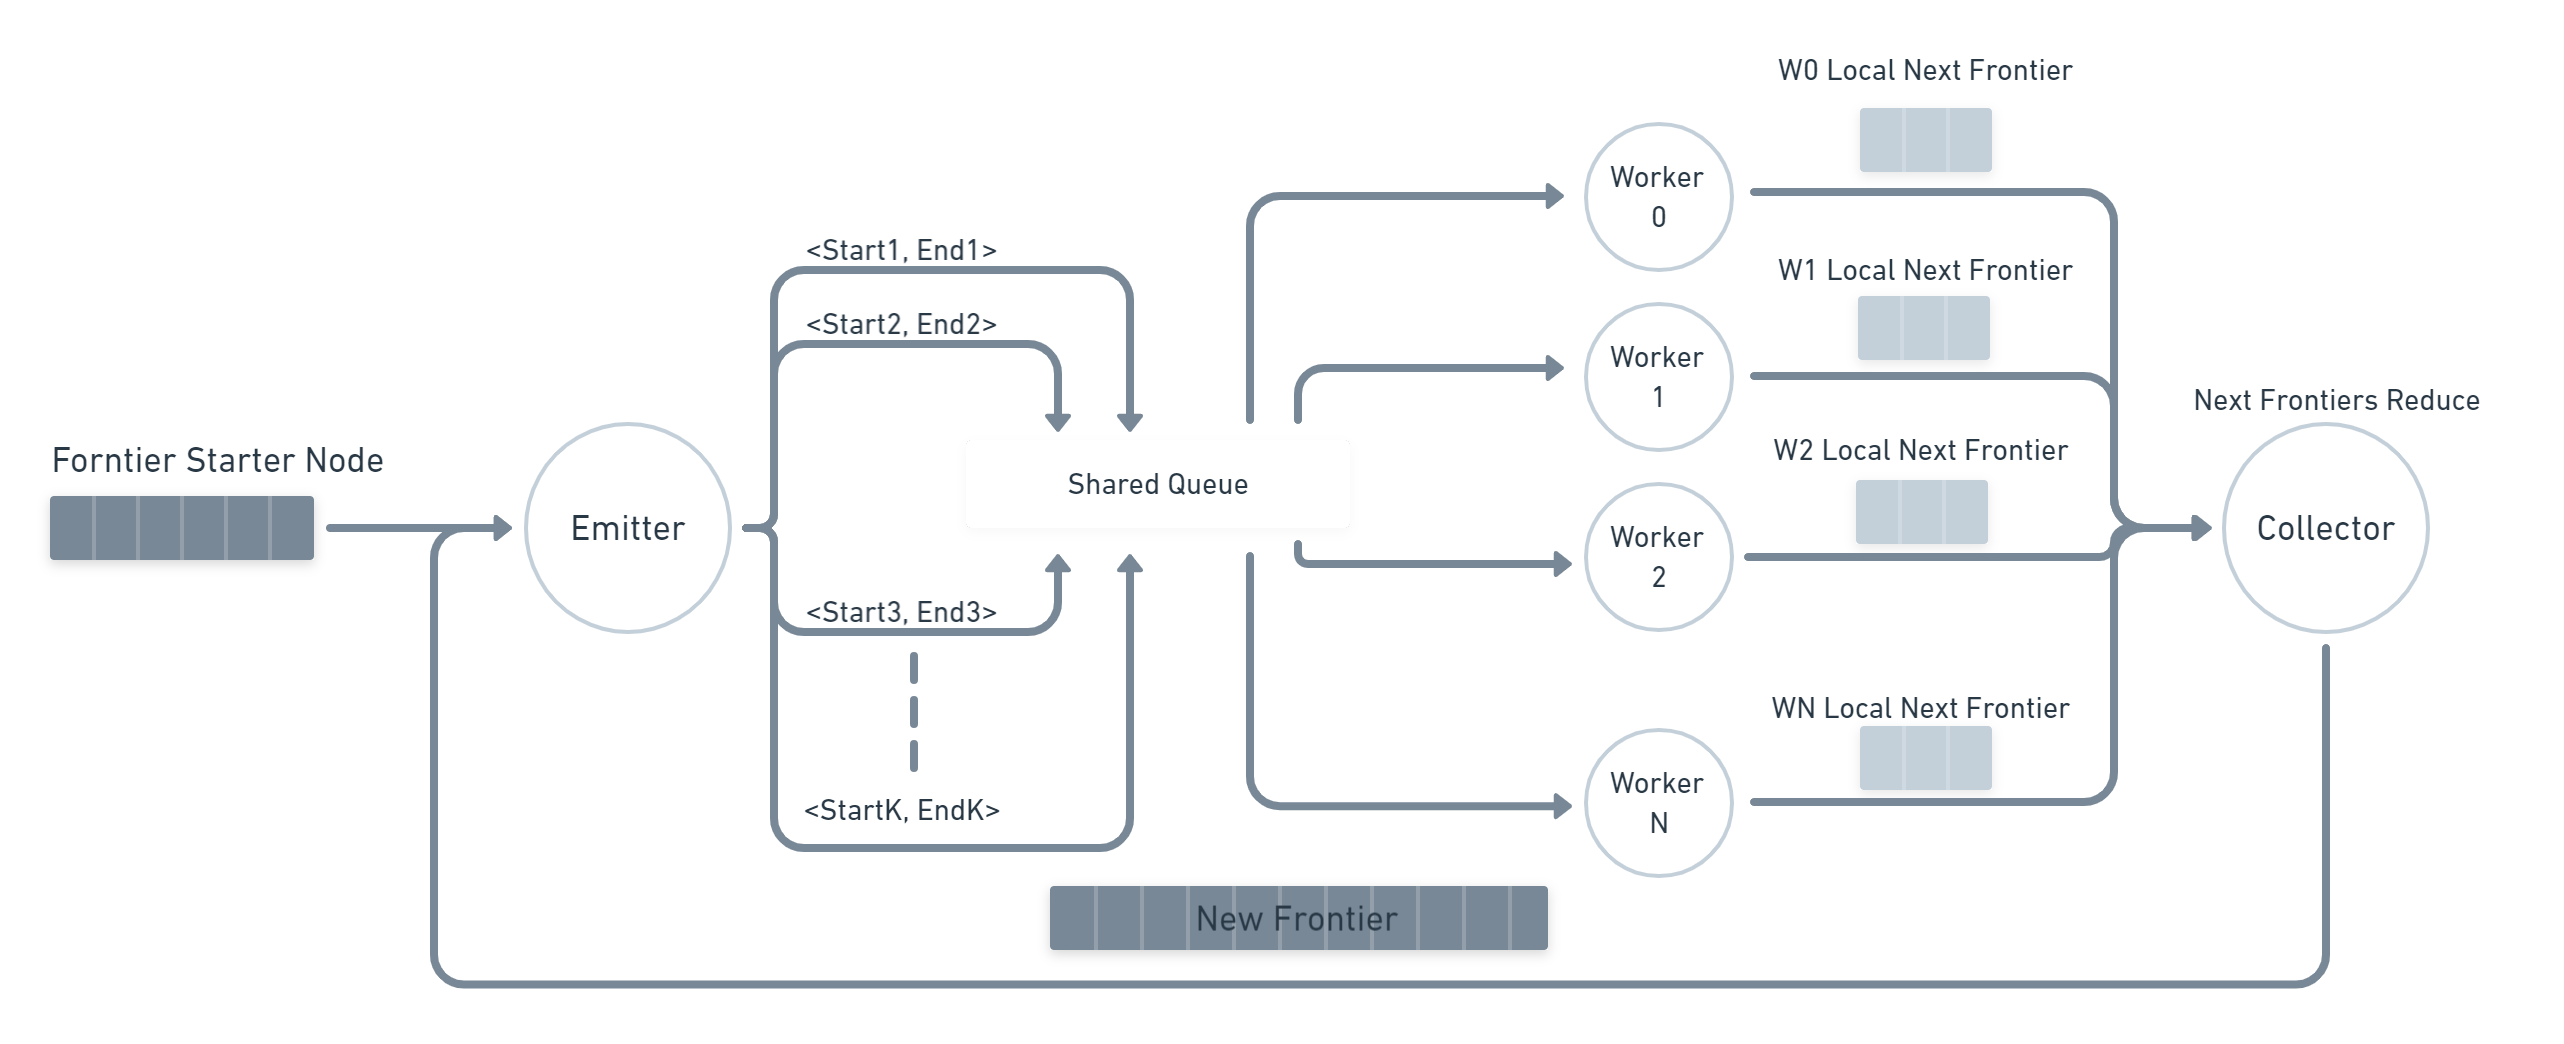
\includegraphics[width=0.95\textwidth]{Figures/par_dy.png}
    \caption{Schema of the dynamic scheduling solution.}
    \label{fig:bfs_par_2_schema}
\end{figure}
\FloatBarrier

Using a dynamic approach for task management the load balancing is distributed evenly across threads as can be seen in the table \ref{table:sched_dy}.
\label{table:sched_dy}
\begin{table}[htb!]
\centering
\begin{tabular}{l|c|c|c|}
\cline{2-4}
\multicolumn{1}{c|}{}                  & Worker 1 & Worker 2 & Worker 3 \\ \hline
\multicolumn{1}{|l|}{Time ($\mu sec$)}             & 23121    & 23376    & 22797    \\ \hline
\multicolumn{1}{|l|}{Discovered nodes} & 2543     & 3376     & 578      \\ \hline
\end{tabular}
\caption{Load balancing of analysis, with dynamic scheduling, of the first frontier graph 10K 0.5 density}
\end{table}

The considerable gain in terms of load balancing removing the bottlenecks in the execution of the farm is counterbalanced by a increase time of the emitter $T_e$, as can been seen in the following tables \ref{table:emit_coll} and \ref{table:emit_coll_dy}.

\begin{table}[!htb]
\centering
\begin{minipage}{0.08\textwidth}
\centering
\begin{tabular}{|c|}
\hline
NW \\ \hline
1          \\ \hline
2      \\ \hline
4           \\ \hline
8            \\ \hline
16       \\ \hline
32          \\ \hline
\end{tabular}
\end{minipage}
\begin{minipage}{0.43\textwidth}
\centering
\begin{tabular}{|c|c|c|}
\hline
 10K 0.02D & 10K 0.5D & 10K 0.8D \\ \hline
 398       & 411      & 552      \\ \hline
905       & 325      & 47       \\ \hline
 1299      & 665      & 466      \\ \hline
1091      & 1284     & 1738     \\ \hline
1524      & 712      & 1524     \\ \hline
1631      & 1460     & 1464     \\ \hline
\end{tabular}

\end{minipage}
\begin{minipage}{0.43\textwidth}
\centering
\begin{tabular}{|c|c|c|}
\hline
 10K 0.02D & 10K 0.5D & 10K 0.8D \\ \hline
149       & 126      & 38       \\ \hline
238       & 149      & 898      \\ \hline
270       & 330      & 77       \\ \hline
290       & 171      & 77       \\ \hline
359       & 230      & 359      \\ \hline
461       & 335      & 52       \\ \hline
\end{tabular}
\end{minipage}
\caption{Total time ($\mu sec$) spend by Emitter and Collector in $\mu sec$, static solution.}
\label{table:emit_coll}
\end{table}

\begin{table}[!htb]
\centering
\begin{minipage}{0.08\textwidth}
\centering
\begin{tabular}{|c|}
\hline
NW \\ \hline
1          \\ \hline
2      \\ \hline
4           \\ \hline
8            \\ \hline
16       \\ \hline
32          \\ \hline
\end{tabular}
\end{minipage}
\begin{minipage}{0.43\textwidth}
\centering
\begin{tabular}{|c|c|c|}
\hline
10K 0.02D & 10K 0.5D & 10K 0.8D \\ \hline
1137       & 565      & 602      \\ \hline
1524       & 1091     & 899      \\ \hline
1465       & 2014     & 1131     \\ \hline
2398      & 905      & 2120     \\ \hline
2614      & 2211     & 1047     \\ \hline
7947      & 6751     & 3645     \\ \hline
\end{tabular}
\end{minipage}
\begin{minipage}{0.43\textwidth}
\centering
\begin{tabular}{|c|c|c|}
\hline
10K 0.02D & 10K 0.5D & 10K 0.8D \\ \hline
111       & 78       & 24       \\ \hline
244       & 103      & 26       \\ \hline
211       & 102      & 49       \\ \hline
214       & 278      & 85       \\ \hline
162       & 119      & 47       \\ \hline
188       & 165      & 75       \\ \hline
\end{tabular}
\end{minipage}
\caption{Total time ($\mu sec$) spend by Emitter and Collector in $\mu sec$, dynamic solution with 32 of chunk size.}
\label{table:emit_coll_dy}
\end{table}
\FloatBarrier


\subsection{Fast Flow Solution}
The Fast Flow solution is based on the same reasoning of the first C++ STL solution (\ref{subsec:CStatic}), in particular, it has been implemented using a farm in which has been removed the collector and added for each worker feedback channel to the emitter. For data communication has been used a personalized task struct in which is present a pair that indicates the start and the end position of the chunk and a next frontier vector. Similar to the first C++ version,  the load balancing is static but in this case, the scheduling exploits the Round Robin algorithm embedded in Fast Flow.

\begin{figure}[htb!]
    \centering
    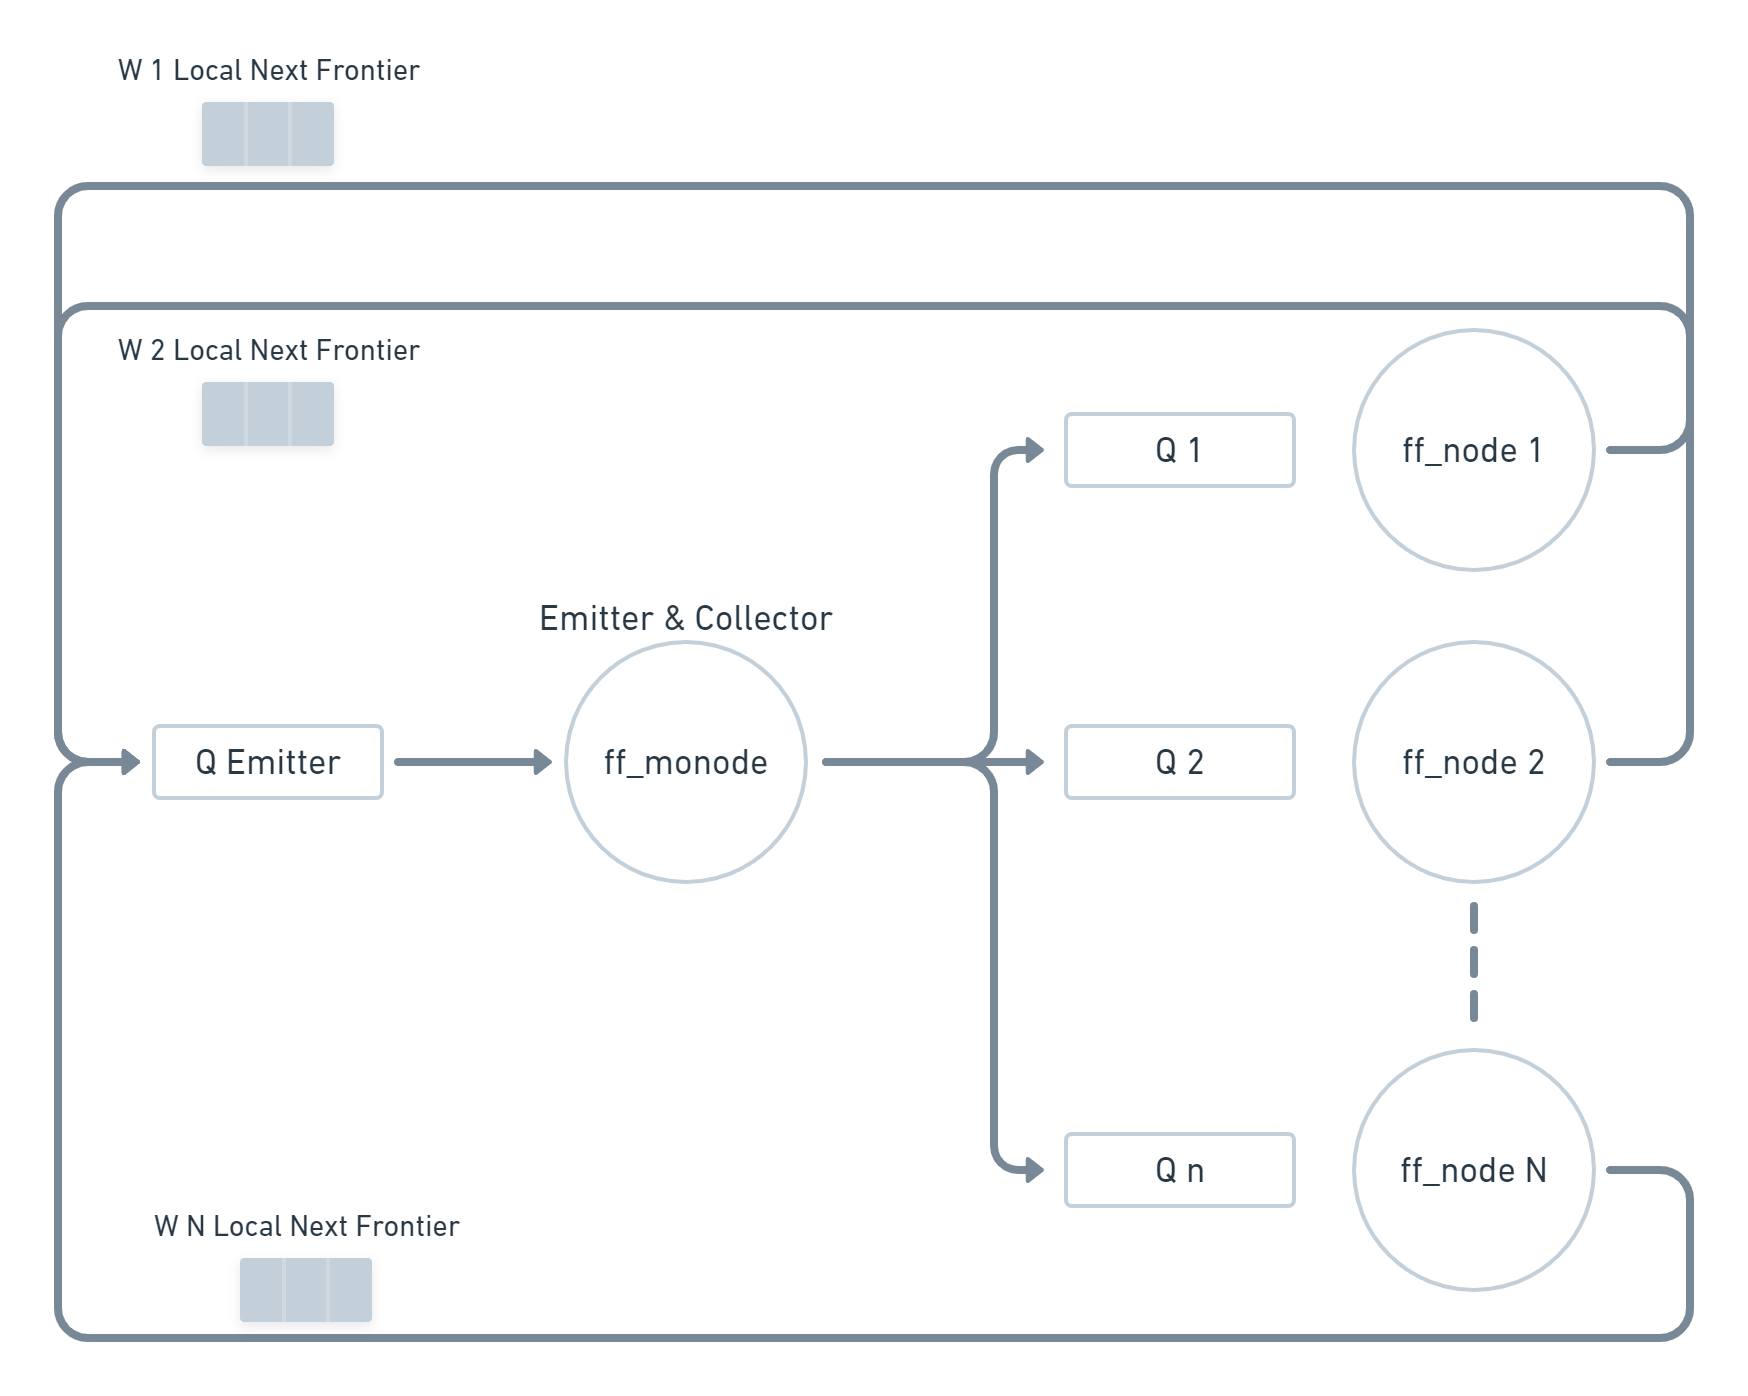
\includegraphics[width=0.75\textwidth]{Figures/FF.png}
    \caption{Schema of the dynamic scheduling solution.}
    \label{fig:FF}
\end{figure}
\FloatBarrier


\section{Results Analysis}
\label{ch:results}
In this section, the results obtained will be shown and compared. Each solution was tested on the proposed graphs in \ref{sec:graph} to verify their behavior in different contexts. 
The test has been executed on \textbf{Xeon PHI}, with $64$ cores and $4$ hardware thread per core. 

In the table (\ref{table:seq_times}) below, are included the sequential times used in the plots and to compute the speedup of the various solutions.
\begin{table}[htb!]
\centering
\begin{tabular}{|c|c|c|c|}
\hline
Sequential & 10K 0.02D & 10K 0.5D & 10K 0.8D \\ \hline
Time ($\mu sec$)          & 21964     & 162399   & 359583   \\ \hline
\end{tabular}
\caption{Time results of the sequential executions.}
\label{table:seq_times}
\end{table}
\FloatBarrier

The following plots show the performance trend of the proposed solutions, starting from the low dense graph.
In this first graph, with density equal to $0.02$, all the four solution have the same behavior also for the performance drop around the $10$ workers. Moreover, the dynamic solution with chunk size of $128$ the knee point comes before due the smaller size of the frontiers.
\begin{figure}[htb!]
    \centering
    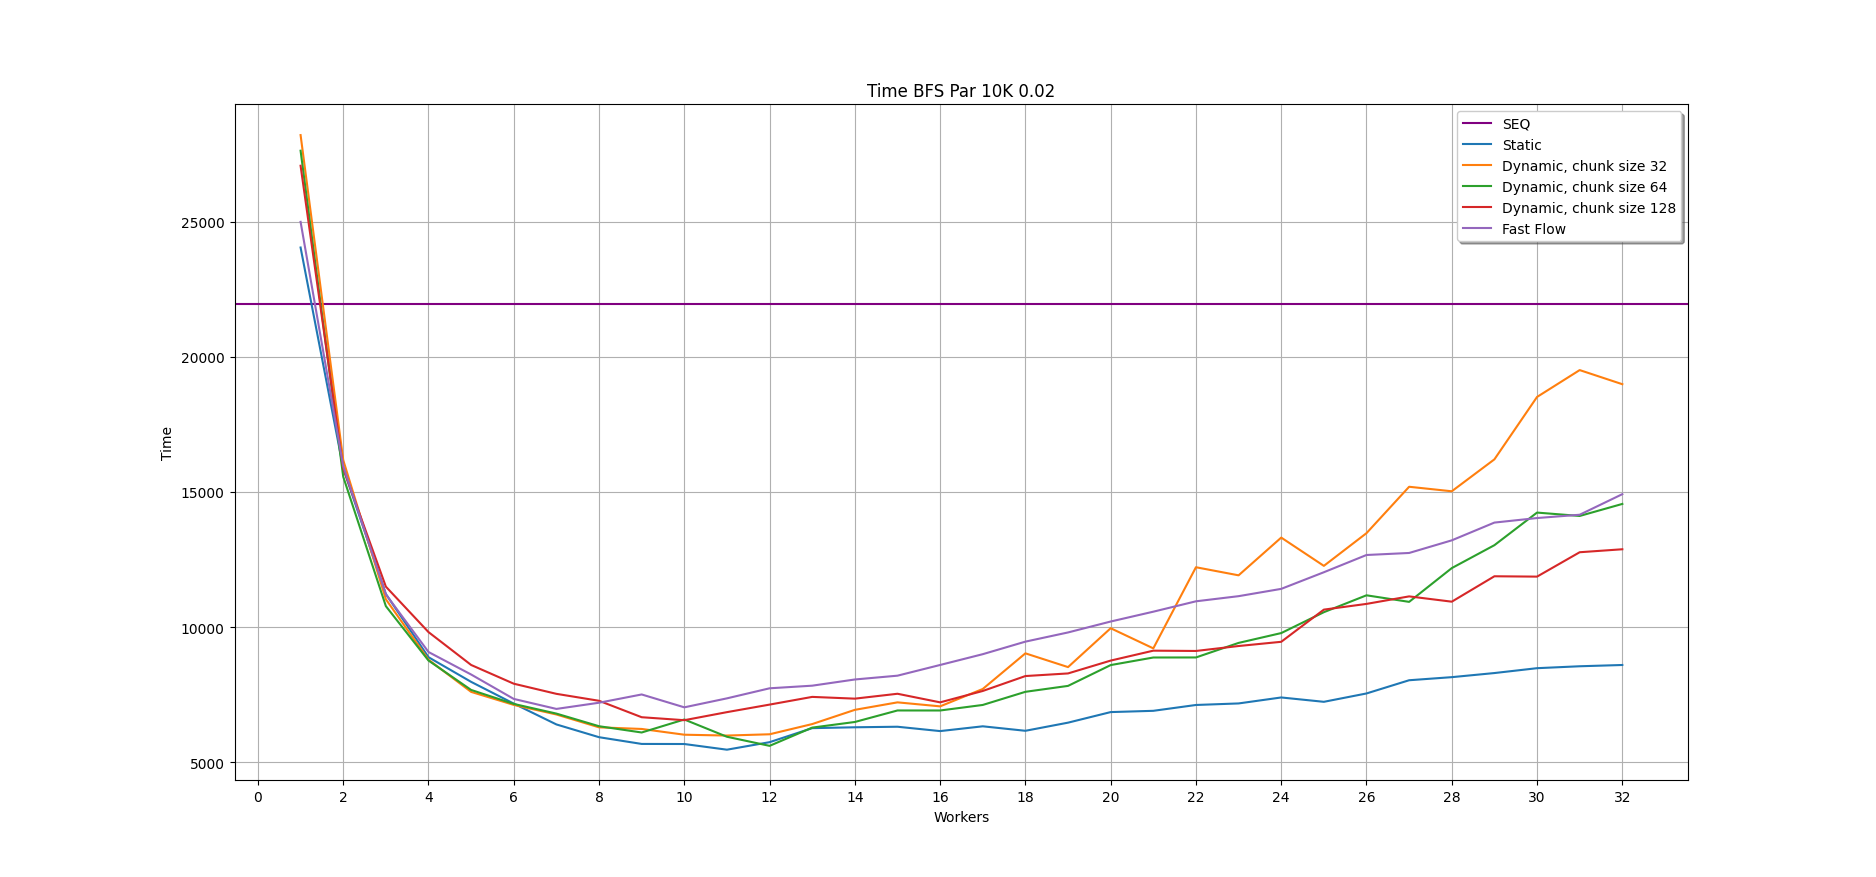
\includegraphics[width=0.75\textwidth]{Figures/plot_map_time_vs10K002.png}
    \caption{Time plot graph 0.02 density.}
    \label{fig:plot_time_10k_002}
\end{figure}
\FloatBarrier

\begin{figure}[htb!]
    \centering
    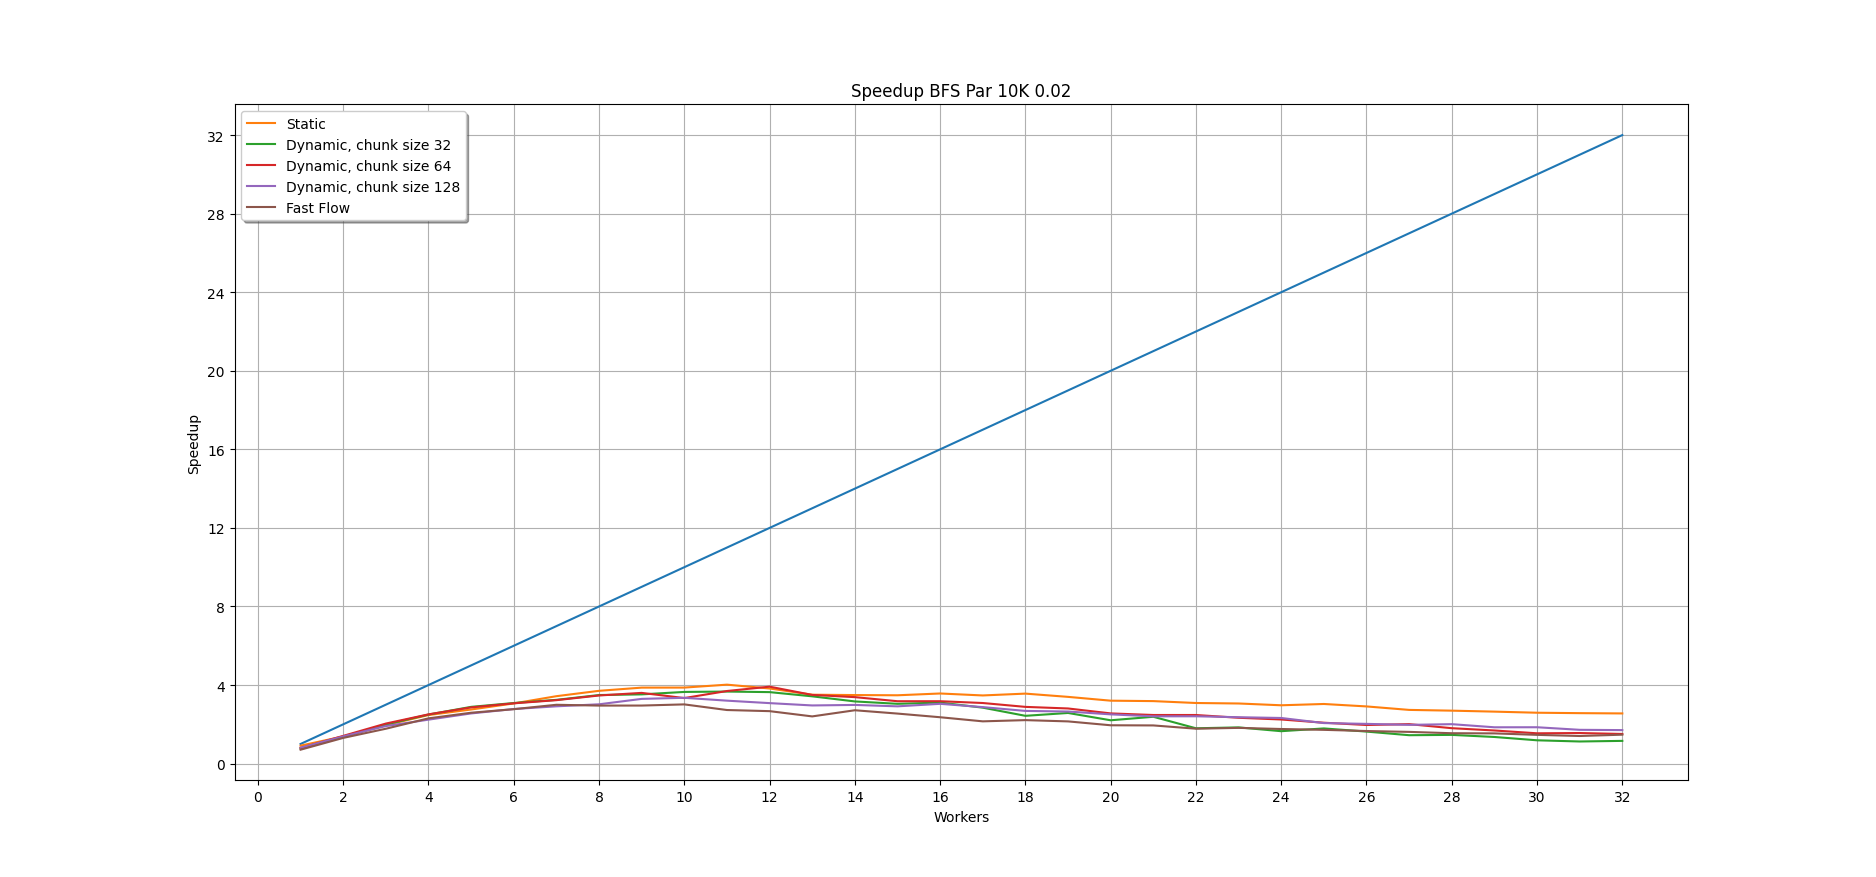
\includegraphics[width=0.75\textwidth]{Figures/plot_map_speedup_vs10K002.png}
    \caption{Speedup plot graph 0.02 density.}
    \label{fig:plot_speedup_10k_002}
\end{figure}
\FloatBarrier
Growing density to $0.5$, and so the frontier size, the static version starts to suffer of load balancing problems mainly in with lower $nw$. Indeed, static approaches, the speedup growth is limited by the large size of the chunks that give the possibility to the first workers to visit most of the graph nodes creating a bottleneck. Meanwhile, dividing the frontier in smaller chunks provides the possibility to handle efficiently the free workers. 

\begin{figure}[htb!]
    \centering
    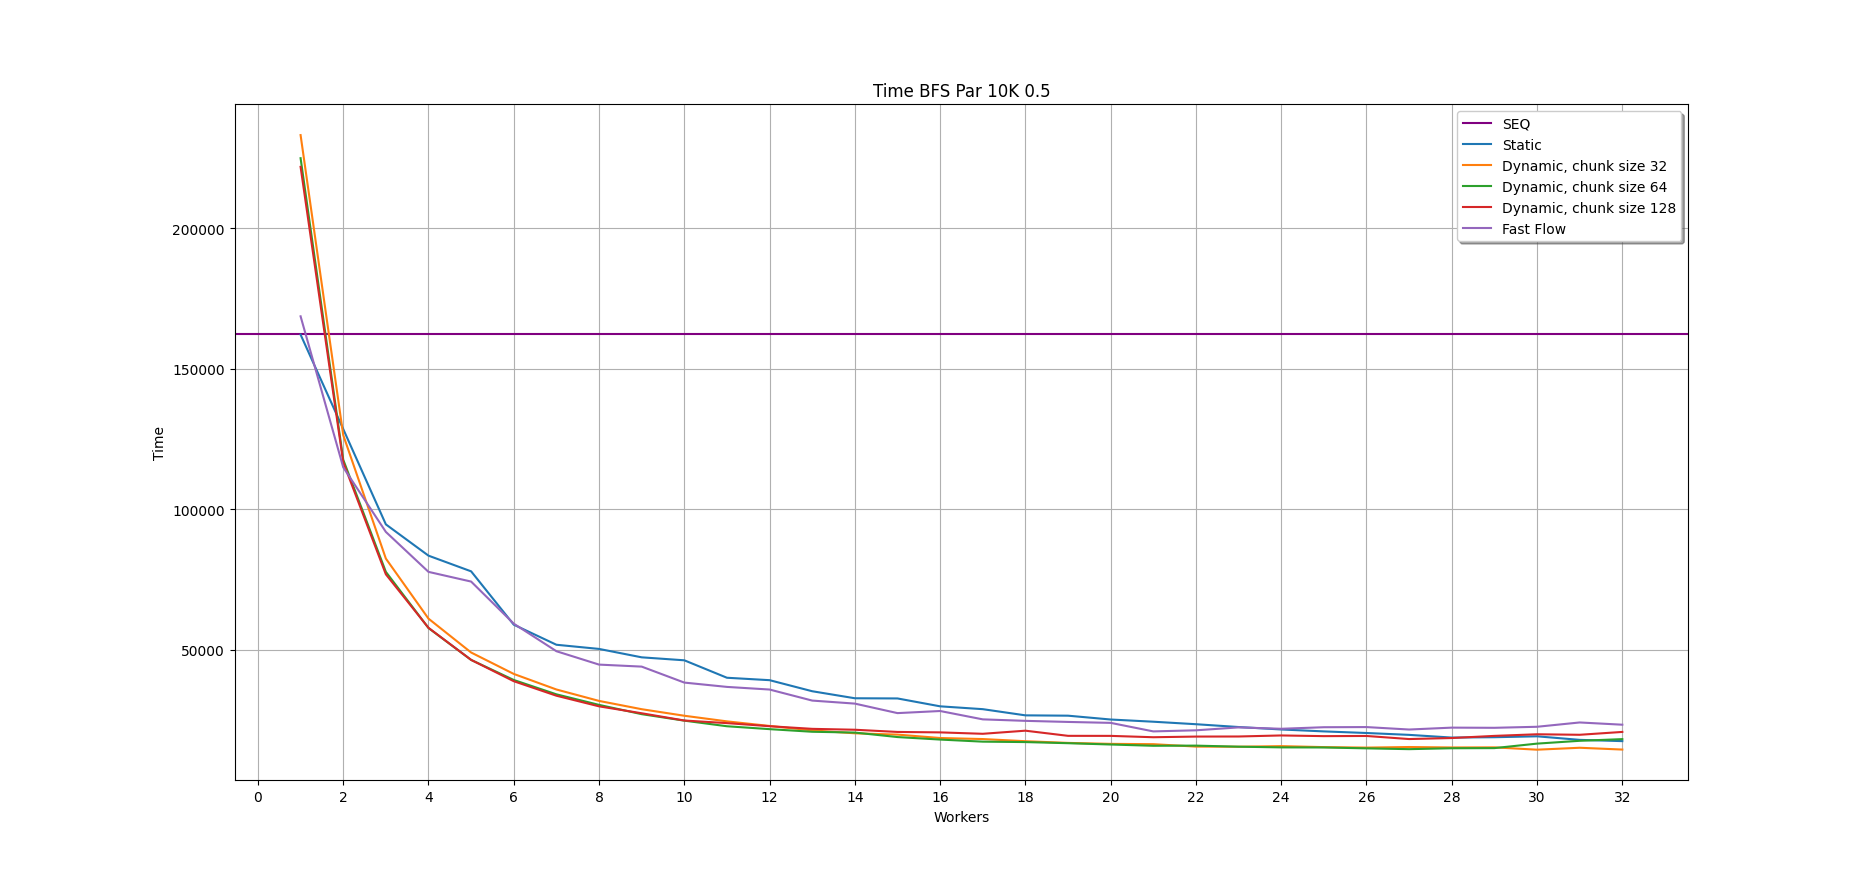
\includegraphics[width=0.75\textwidth]{Figures/plot_map_time_vs10K05.png}
    \caption{Time plot graph 0.5 density.}
    \label{fig:plot_time_10k_05}
\end{figure}
\FloatBarrier

\begin{figure}[htb!]
    \centering
    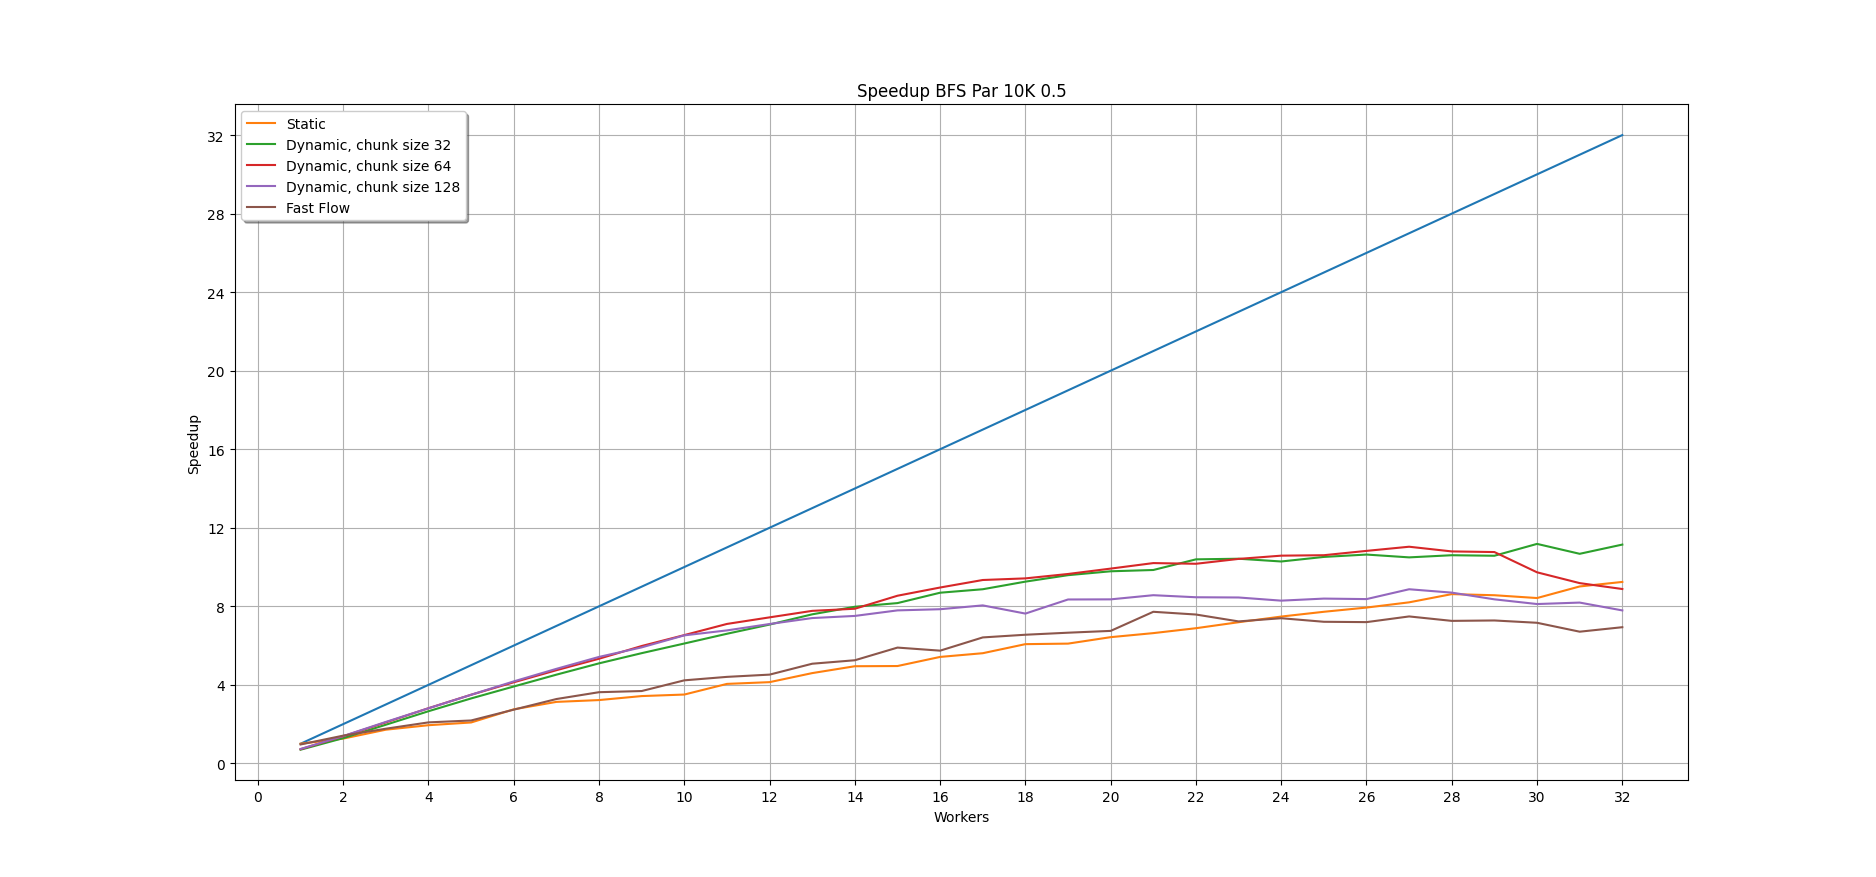
\includegraphics[width=0.75\textwidth]{Figures/plot_map_speedup_vs10K05.png}
    \caption{Speedup plot graph 0.5 density.}
    \label{fig:plot_speedup_10k_05}
\end{figure}
\FloatBarrier

The analysis of the last graph is almost the same and also in this case the Fast Flow version maintains a speedup margin about one point less than the version with static scheduling. This could be due to the task management by fast flow and for runs with many threads the need to re-execute $nw$ times the $svc$ method of the emitter with related checks. Also, for each new level of the graph the tasks are not reused but new ones are created, for very large frontiers this is a considerable overhead compared to the emitter in other versions (see table \ref{table:emit_coll}).

\begin{figure}[htb!]
    \centering
    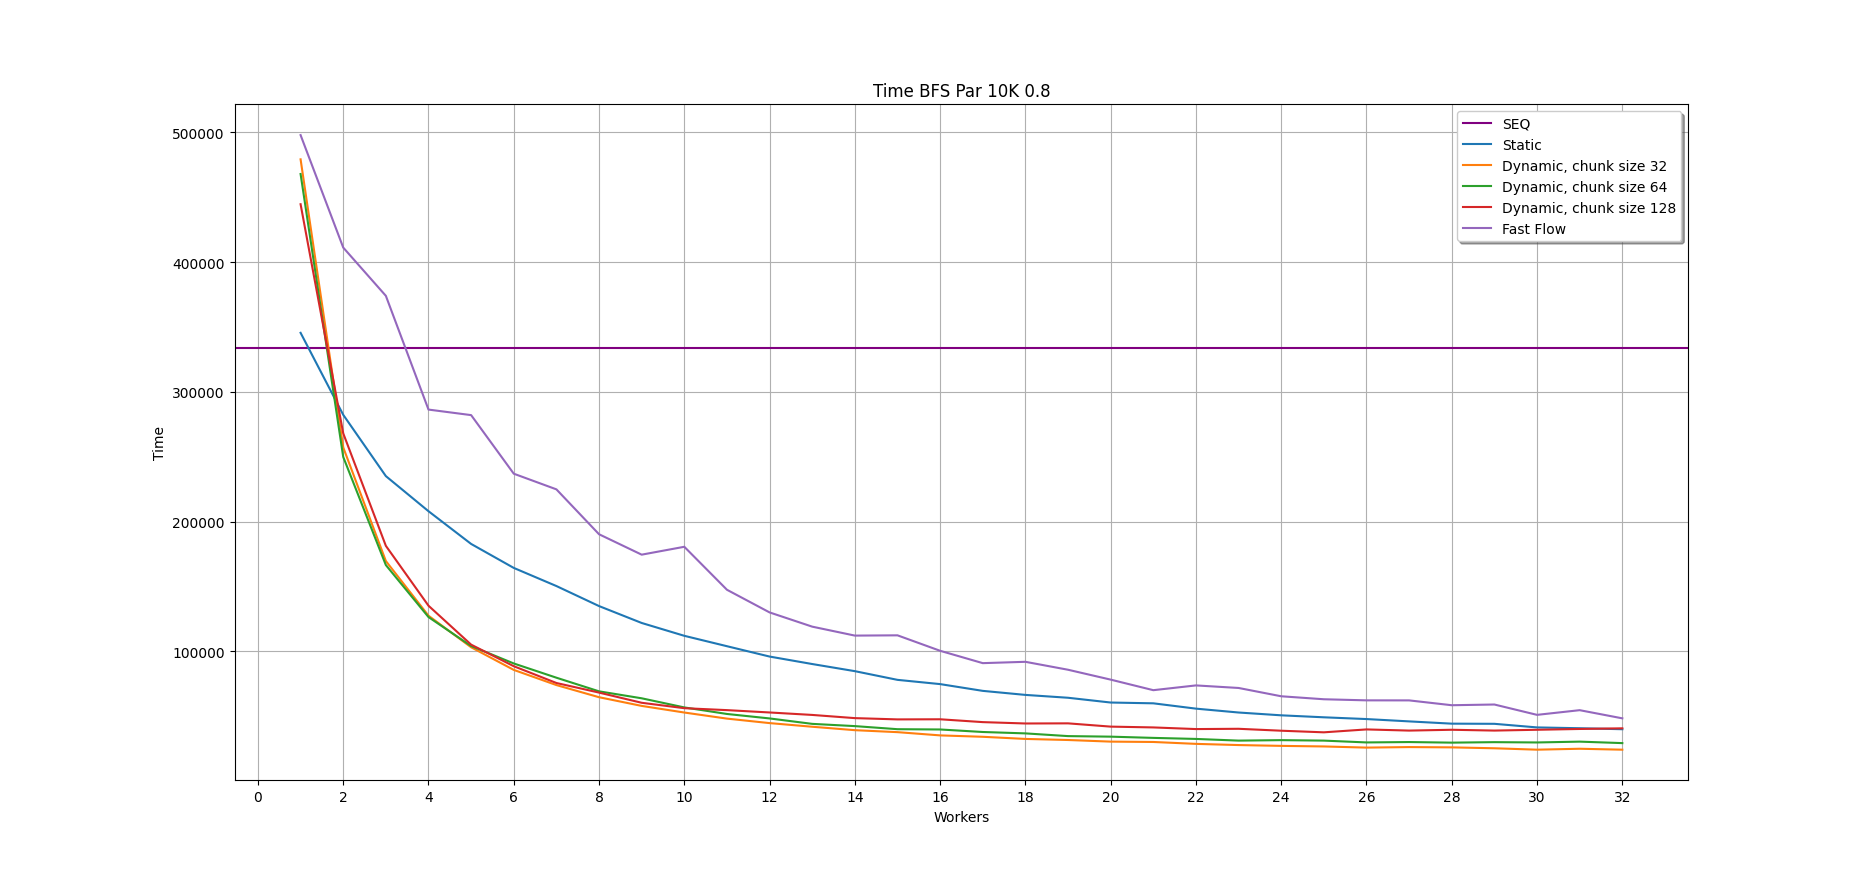
\includegraphics[width=0.75\textwidth]{Figures/plot_map_time_vs10K08.png}
    \caption{Time plot graph 0.8 density.}
    \label{fig:plot_time_10k_08}
\end{figure}
\FloatBarrier

\begin{figure}[htb!]
    \centering
    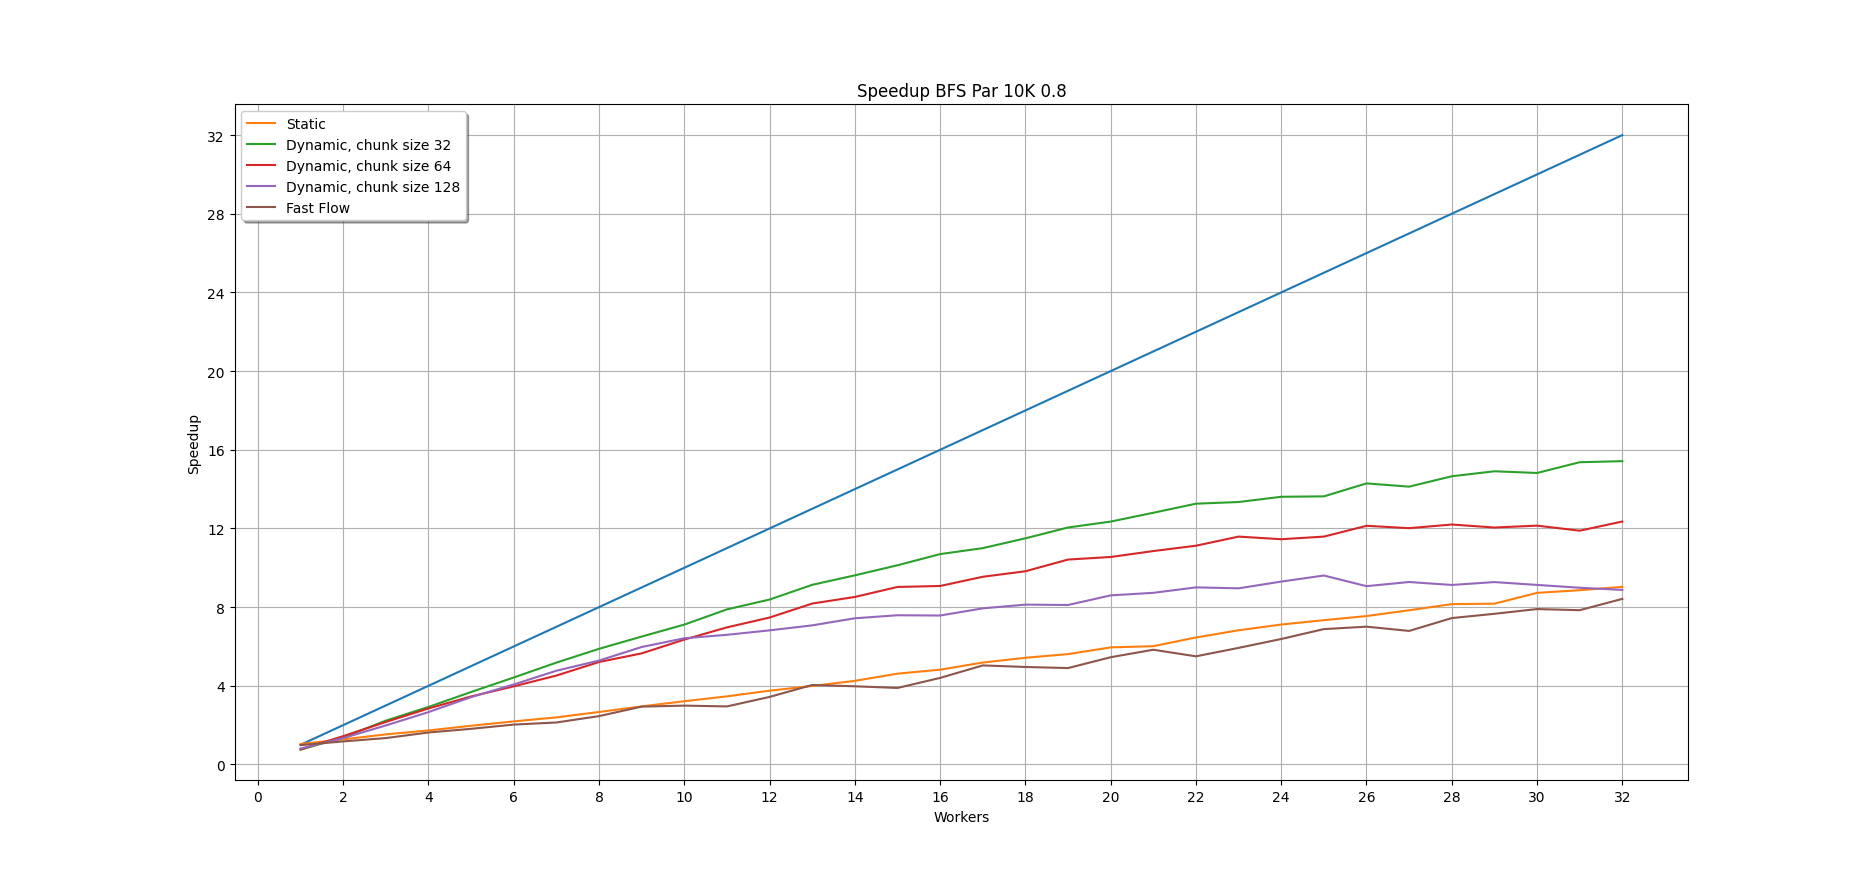
\includegraphics[width=0.75\textwidth]{Figures/plot_map_speedup_vs10K08.png}
    \caption{Speedup plot graph 0.8 density.}
    \label{fig:plot_speedup_10k_08}
\end{figure}
\FloatBarrier
In the following tables you can see the speedup trend from a numerical point of view for all versions.
\begin{table}[htb!]
\centering
\begin{tabular}{|c|c|c|c|}
\hline
Workers & 10K 0.02D & 10K 0.5D & 10K 0.8D \\ \hline
1       & 0,913606  & 1,001233 & 1,040779 \\ \hline
2       & 1,383123  & 1,262705 & 1,273857 \\ \hline
4       & 2,471753  & 1,943502 & 1,729321 \\ \hline
8       & 3,705753  & 3,223546 & 2,667787 \\ \hline
16      & 3,569641  & 5,421432 & 4,819437 \\ \hline
32      & 2,554548  & 9,240867 & 9,029531 \\ \hline
\end{tabular}
\caption{Speedup static scheduling.}
\label{table:spup_static}
\end{table}
\FloatBarrier

\begin{table}[]
\centering
\begin{tabular}{|c|c|c|c|}
\hline
Workers & 10K 0.02D & 10K 0.5D & 10K 0.8D \\ \hline
1       & 0,708265  & 0,703803 & 0,791419 \\ \hline
2       & 1,308471  & 0,961453 & 0,943141 \\ \hline
4       & 2,303997  & 1,328917 & 1,39952  \\ \hline
8       & 2,953739  & 2,382475 & 2,059774 \\ \hline
16      & 2,360451  & 3,646711 & 3,770874 \\ \hline
32      & 1,472611  & 5,801207 & 7,44725  \\ \hline
\end{tabular}
\caption{Speedup Fast Flow solution.}
\label{table:spup_ff}
\end{table}
\FloatBarrier

\begin{table}[htb!]
\centering
\begin{tabular}{|c|c|c|c|}
\hline
Workers & 10K 0.02D & 10K 0.5D & 10K 0.8D \\ \hline
1       & 0,778865  & 0,696421 & 0,750639 \\ \hline
2       & 1,357478  & 1,284081 & 1,378061 \\ \hline
4       & 2,497896  & 2,655661 & 2,922916 \\ \hline
8       & 3,490782  & 5,093752 & 5,879286 \\ \hline
16      & 3,107527  & 8,691875 & 10,69519 \\ \hline
32      & 1,156913  & 11,14306 & 15,42083 \\ \hline
\end{tabular}
\caption{Speedup dynamic scheduling solution with chunk size of 32 nodes.}
\label{table:spup_dy}
\end{table}
\FloatBarrier
\newpage

\section{Conclusion}
\label{ch:conclusion}
In the report,  the Breadth-First Search algorithm has been analyzed and some possible parallel solutions to improve the performance of the sequential implementation have been proposed.
The problem analysis leads to determine that the frontier visit is the best spot for the parallelization. To achieve it, a farm-based approach has been used, in particular, three solutions were developed: static and dynamic scheduling using pthread and static scheduling with Fast Flow version.

The evaluation of the results shows that with a static partitioning, that splits the frontier based on the number of workers in the farm, presents a worse load balancing. This scenario occurs especially with a low number of workers and with very dense graphs. 
To solve this problem, a dynamic scheduling version has been proposed that allows to divide the level into smaller chunks and using a shared data structure between workers to manage the workload in a more balanced way. 
In Fast Flow the obtained results are very similar to the static pthread version, as they share the same workload management, with a drop in performance for numerous farms that carry a greater overhead due to the communication mechanisms.
The behavior of the solutions on the tested graphs leads to believe that with larger number of nodes it could be possible, in principle, to obtain remarkable speedups, therefore they could be preferred to a sequential version.


%\let\cleardoublepage\clearpage %per togliere solo qui la pagina bianca che si crea
%\renewcommand\bibname{Webography} 
%\begin{thebibliography}{0}
%\setcounter{enumiv}{0} 

%\bibitem{url1} NetworkX
%\url{https://networkx.github.io/}



%\end{thebibliography}
\end{document}